% !TeX encoding = UTF-8

\chapter{INTRODUÇÃO}\label{ch:introducao}

O reconhecimento de face é um dos campos de pesquisa mais interessantes e importantes nas ultimas duas décadas \cite{wei_lun}. Grandes empresas estão na corrida para ver quem desenvolve o melhor algoritmo de reconhecimento de faces, e apenas à pouco tempo, duas delas (Google e Baidu) conseguiram taxas de erros abaixo das apresentadas por seres humanos (que se acera aos 8\%) \cite{stats_economy_compass_2017}.

As possibilidades de uso de um sistema de reconhecimento de faces são vastas (desde o uso comercial como empresas que querem identificar seus clientes e oferecer um serviço personalizado ao uso da polícia para o combate criminal e forense). Chega a ser um assunto polêmico em alguns círculos pois podem inferir em invasão de privacidade e privação da liberdade como a conhecemos.

As pesquisas sobre o assunto envolvem conhecimentos de disciplinas como neurociência, psicologia, computação visual, reconhecimento de padrões, processamento de imagens, matemática avançada \cite{wei_lun}, por isso apresenta um grande problema computacional. Além do problema de manipulação de imagens,  de identificação e reconhecimento das faces, deve-se considerar problemas de persistência destas, a questão de treinamento das faces, velocidade de verificação, de extração de dados de imagens e vídeos (tarefa em que a linguagem Java não tem boa fama) e desempenho em geral. Não houve um grupo de desenvolvedores ou indivíduos capaz de encerrar esse assunto.


\section{BREVE HISTÓRIA}\label{sec:historia}

O reconhecimento automático de faces é um conceito relativamente novo. Desenvolvido na década de 60, o primeiro sistema semi-automático requeria que um administrador do sistema localizasse pontos da imagem como olhos, boca, nariz,  etc, e depois um algorítimos comparava as distâncias entre estes pontos em diferentes fotos para dar um resultado de comparação \cite{nstc_homeland}. Nos anos 80, algorítimos simples foram criados para automatizar este processo. Em 1988, Kirby e Sirovich aplicaram Análise de Componente Principal, uma técnica padrão de álgebra linear, para o problema de reconhecimento de face. Este foi considerado um marco pois mostrou que menos que 100 valores são requeridos para codificar uma imagem de uma face normalizada e bem posicionada \cite{nstc_homeland}. Em 1991, Turk e Pentland descobriu o erro residual das comparações feitas com a técnica \textit{eigenfaces} poderiam ser usadas para detectar faces em uma imagem - uma descoberta que permitiu detecção em tempo-real. Apesar de esta abordagem ser limitada a posição da face, qualidade da imagem e fatores de ambiente, ela criou um significante interesse no desenvolvimento de tecnologias automáticas para reconhecimento \cite{nstc_homeland}. A tecnologia capturou a atenção da mídia e do público em janeiro de 2001 no evento \textit{SuperBowl}, que capturou rostos das imagens das câmeras de vigilância e comparou com fotos digitais "3x4" de uma base de dados apresentando rostos similares \cite{nstc_homeland}.

Hoje, o reconhecimento de faces está sendo usado no combate à fraude de passaportes e cédulas de identidades onde a foto é padronizada com ambiente controlado, aplicativos de celulares e redes sociais para entretenimento, enquanto que grandes governos e organizações patrocinam, incentivam e desafiam empresas para conseguir o algoritmo ideal de reconhecimento \cite{nyu_ccpr_frt}.



\section{PROBLEMÁTICA}\label{sec:problematica}

A face é um objeto 3D que é iluminada por uma grande variedade de fontes de luz e envolvida por um fundo com “dados arbitrários” (inclusive outras faces). Portanto, a aparência que uma face possui quando projetada para um modelo 2D pode variar tremendamente. Na verdade, problemas de iluminação e de segmentação “\textit{foreground-background}” tem sido questões pertinentes no campo da computação gráfica e visual como um todo \cite{tony_columbia}. Sendo assim o primeiro problema a enfrentar seria a aquisição de imagem e suas condições.


\subsection{DETECÇÃO E AQUISIÇÃO DA FACE}\label{subsec:aquisicao_imagem}

Em geral, em uma imagem retirada de vídeo um digital de nível amador, o módulo de identificação da face deve encontrar condições luminosas descontroladas, alta variação de poses, maquiagem, mudanças nos pelos faciais, adoecimento, envelhecimento, oclusões da face por interferência, roupa ou cabelo, enfim, uma incontável gama de variáveis \cite{tony_columbia}. De fato, há diversos desafios e fatores chaves que podem significantemente impactar a performance da identificação e reconhecimento da face e os pontos de verificação (\textit{matching scores}).

Na \autoref{ex_variacao_fig}, lista-se exemplos de alguns destes desafios em imagens, respectivamente:

\begin{figure}[h]
	\centering
	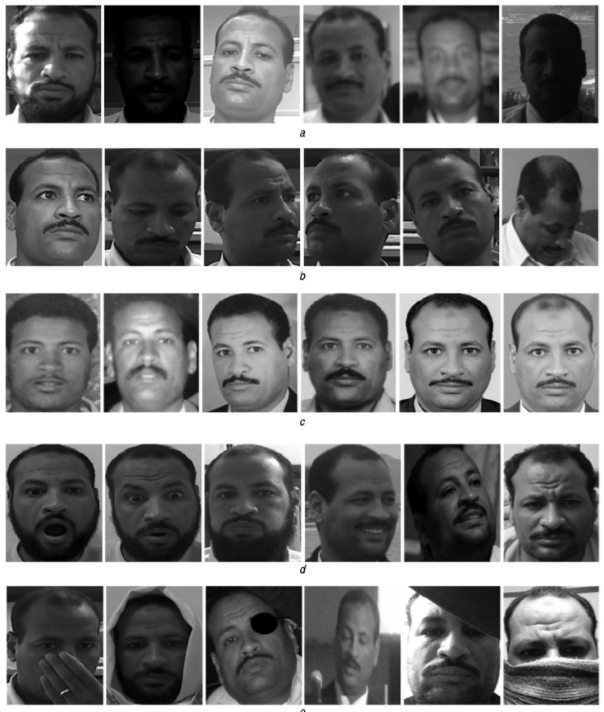
\includegraphics[width=.8\textwidth]{ex_variacao}
	\caption{Exemplos de Variação}
	\fonte{The Reseachgate.net}
	\label{ex_variacao_fig}
\end{figure}


\begin{enumerate}[label=(\alph*)]
	\item Variação de iluminação;
	\item Variação de poses ou pontos de visão;
	\item Envelhecimento;
	\item Expressões faciais e estilo da face (pelos faciais ou maquiagem);
	\item Oclusão.
\end{enumerate}


A aquisição de faces em vídeos (diz-se \textit{tracking} ou rastreamento) segue a mesma lógica e tem os mesmo problemas de aquisições de faces estáticas. O rastreamento nada mais é do que a detecção contínua da face em \textit{frames} advindos de um vídeo, com um forte problema adicional de que deve-se manter a usabilidade do sistema em um computador contemporâneo de baixa a média performance. Em outras palavras, o processamento envolvido deve ser eficiente o bastante considerando o tempo de execução do vídeo (\textit{frames} por segundo) e do sistema e tempo de armazenamento e consulta de dados.

A performance da detecção da face é uma questão-chave no processo de reconhecimento, porém considerada bem para poses de faces frontais, deste a década de 90. A detecção de faces pode ser considerada um caso específico da área de detecção de objetos, alcançando confiáveis \cite{stats_face_detection_IEEE}.

Em um trabalho feito em 2003 por \cite{final_project_stanford} na Universidade de Stanford - Califórnia, utilizaram a técnica \textit{EigenFaces} para detecção, acrescido de algorítimo de identificação de gênero de sexo, com um \textit{Pentium 3} de 700 Mhz e menos de 500 megas de memória, alcançaram resultados que superam 93\% de taxa de sucesso nas condições mais adversas, considerando iluminação e escala (numero grande de faces em uma imagem). Outros \textit{benchmarks} mais recentes (2015) apresentam resultados que superam os 97.2\% \cite{stats_hong_kong}.

O problema com estas técnicas relativamente antigas, é que também reconhecem fotos de fotos, ou desenhos de faces como legítimas faces, por vezes até com pontuação bastante para uma verificação de sucesso com uma face real. Outro problema é estas técnicas não funcionam num angulo de perfil, ou de qualquer outro ângulo que não seja o frontal.

Novas técnicas de detecção não-frontais estão sendo implementadas, bem como as de modelagem sub-espacial 3D e comparações com reconhecimento de padrões baseados em aprendizado de máquinas e redes neurais, são fundamentos para os sistemas de reconhecimento de face avançados, capazes de reconhecer não só a face, mas também a estrutura cranial do alvo \cite{3dmodel_fd}. 

Após a face ser identificada e localizada na imagem, para que sirva ao processo de reconhecimento, deve-se recortar esta face da imagem e performar algumas operações gráficas sobre a mesma. Nesta fase são consideradas atividades de corte da face na região localizada, escalamento e correção de rotação, transformar em preto e branco, normalizar a imagem para minimizar as condições de ambiente da foto, deixando a face pronta para a próxima faze do processo: o treinamento.


\subsection{TREINAMENTO E RECONHECIMENTO DA FACE} 

Esta fase consiste em manipular a face recortada da imagem ou \textit{frame} e já normalizada e tratada de forma a extrair informações e características desta para que se possa salvar de alguma forma e relacionar estas características com a pessoa ou alvo. Nesta fase é importante aquisitar fotos da mesma face mostrando diferentes expressões faciais e situações de lumiosidade e posição.

A forma que isso pode ser feito depende totalmente do algorítimo de reconhecimento envolvido. Há várias técnicas e algorítimos de reconhecimento, como \cite{issues_methods_FR}:

\begin{itemize}
	\item reconhecimento baseado em redes neurais;
	\item reconhecimento baseado em processamento 3D;
	\item reconhecimento baseado em descritores de face;
	\item reconhecimento baseado em reconstrução;
	\item reconhecimentos tradicionais ou clássicos, dentre outros;
\end{itemize}

Este trabalho se focará em dois dos algorítimos clássicos, famosos por serem pioneiros e objetos de muito estudo, testes e documentação: \textit{EngenFaces} e \textit{FisherFaces}. Os algorítimos convencionais podem ser divididos em duas categorias: caracterização holística ou linear, sendo que \textit{EngenFaces} e \textit{FisherFaces} fazem parte da primeira, que fazem parte de outra subdivisão de métodos de projeção linear chamada Análise de Componentes Principais - ACP (ou no inglês, Principal Component Analysis – PCA) \cite{issues_methods_FR}.

Basicamente, o método ACP consiste em tratar a imagem de uma forma uniforme, coletar características da mesma transformando-as em valores numéricos e disponibilizá-las em um plano cartesiano, que pode ter mais de três dimensões. Este processo visa destacar discrepâncias da face, ou seja, padrões de mudança de constaste, de relevo ou sombreamentos, ou diferença de cores. A transformação destes valores manipulados de volta em imagens, cria os chamados \textit{EngenFaces} (Faces de fantasmas, em Alemão), pois como mustra a \autoref{someeigen}, é devido a sua estranha aparência \cite{drmathew_java_programming}.

\begin{figure}[h]
	\centering
	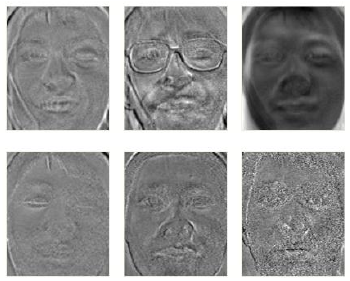
\includegraphics[width=.6\textwidth]{someeigen}
	\caption{Exemplos de EigenFaces}
	\fonte{\cite{drmathew_java_programming}}
	\label{someeigen}
\end{figure}

A ideia é quem uma imagem de treinamento pode ser decomposta em uma soma multiplas \textit{eigenfaces} medidas e disponibilizadas em uma sequencia especial.

Uma maneira mais simples de representar o relacionamento entre \textit{eigenfaces} e imagens das faces é quem estas faces são disponibilizadas em um espaço multidimensional, ou um plano cartesiado "n" dimensões onde os eixos do plano são as \textit{eigenfaces} \cite{drmathew_java_programming} como ilustra a  \autoref{eigencartesiano}.

Tendo a face (ou faces) relacionada com o alvo, representado em valores e disponibilizada em um plano cartesiano de “n” dimensões, resta a verificação ou reconhecimento da face contra outra. 

Para o reconhecimento da face propriamente dito, o mesmo processo do treinamento deve ser repetido e a face representada e disponibilizada no mesmo plano cartesiano das faces treinadas \cite{drmathew_java_programming}. A distancia entre as duas faces representadas no plano cartesiano é medida, e basicamente, quando menor a distância, maior é a taxa de reconhecimento. Ou seja, uma distância zero entre as duas faces representadas no plano seria uma correspondência perfeita. A \autoref{eigencartesiano} abaixo ilustra esta descrição:

\begin{figure}[h]
	\centering
	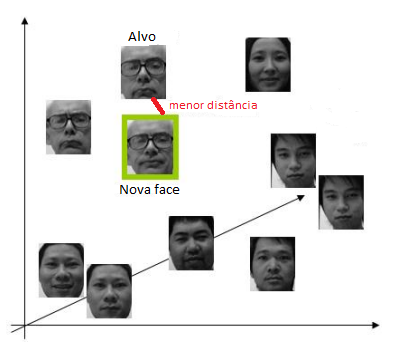
\includegraphics[width=.6\textwidth]{eigencartesiano}
	\caption{Exemplos de EigenFaces}
	\fonte{Adaptado de \cite{drmathew_java_programming}}
	\label{eigencartesiano}
\end{figure}

Este plano cartesiano, na prática, pode ser um arquivo binário ou texto, comumente chamado de "\textit{bundle}".

\section{OBJETIVOS}\label{sec:objetivos}
Este projeto propõe a implementação de um Sistema de Reconhecimento de Faces em Vídeo utilizando dois dos primeiros algorítimos desenvolvidos para este fim: \textit{FisherFaces} e \textit{EigenFaces}.

O algorítimo \textit{EigenFaces} será implementato seguindo as instruções e exemplois de código de \cite{drmathew_java_programming}. Quanto ao algoritmo \textit{FishFaces}, será usado a implementação da biblioteca OpenCV. Haverá uma tentativa de fazer com que os dois algorítimos funcionem juntos para que se use os pontos fortes de cada um, eliminando os fracos, e se possível melhorar a taxa de reconhecimento. 

\subsection{ORGANIZAÇÃO DO TRABALHO}\label{sec:organizacao-trabalho}

O desenvolvimento do sistema, basicamente, se fará na exploração das seguintes fases:

\begin{itemize}
	\item Análise das bibliotecas e suas versões para melhor escolha;
	\item Preparação do ambiente;
	\item Implementação da interace e manipulação de imagens (e vídeos)  utilizando componentes Java e as bibliotecas gráficas (para  recorte de frames e imagens, aplicação de filtros, mineração de dados da imagem, manipulação de cores, iluminação, normalização, etc);
	\item Implementação do algorítimo EigenFaces;
	\item Detecção de face em imagens tiradas com câmera;
	\item Treinamento / reconhecimento de face na imagem;
	\item Incrementar a implementação feita acima para o treinamento  e reconhecimento em vídeo tirado da câmera em tempo real;
	\item Integrar os algorítimos de outras implementações;
	\item Performar uma bateria de testes, e comparar resultados.
\end{itemize}

O objetivo final é estruturar todas esta pesquisa e o respaldo técnico que desses algorítimos, contemplar problemas tecnológicos da linguagem JAVA e de ambiente de desenvolvimento e a partir disso criar um sistema de reconhecimento de faces em vídeo, analisando seus resultados e disponibilizar a pesquisa e anotações para fins didáticos, finalmente disponibilizando todo o trabalho e o código aberto ao público desenvolvedor e acadêmico.


\subsection{JUSTIFICATIVA} 

O reconhecimento de faces é umas das tecnologias mais estudadas e complexas de hoje em dia. As maiores empresas e governos do planeta estão na corrida para se acercarem aos 100\% de acerto em seus reconhecimentos e governos e organizações como FBI e NSA investem e desafiam os produtores desta tecnologia \cite{nstc_homeland}.

Eis na \autoref{tabelaempresasrecog} algumas das empresas quem produzem tecnologias de reconhecimento de ponta:

\vspace*{5cm}
\begin{table}[h]
	\centering
	\caption{Empresas que produzem tecnologias de reconhecimento de faces}
	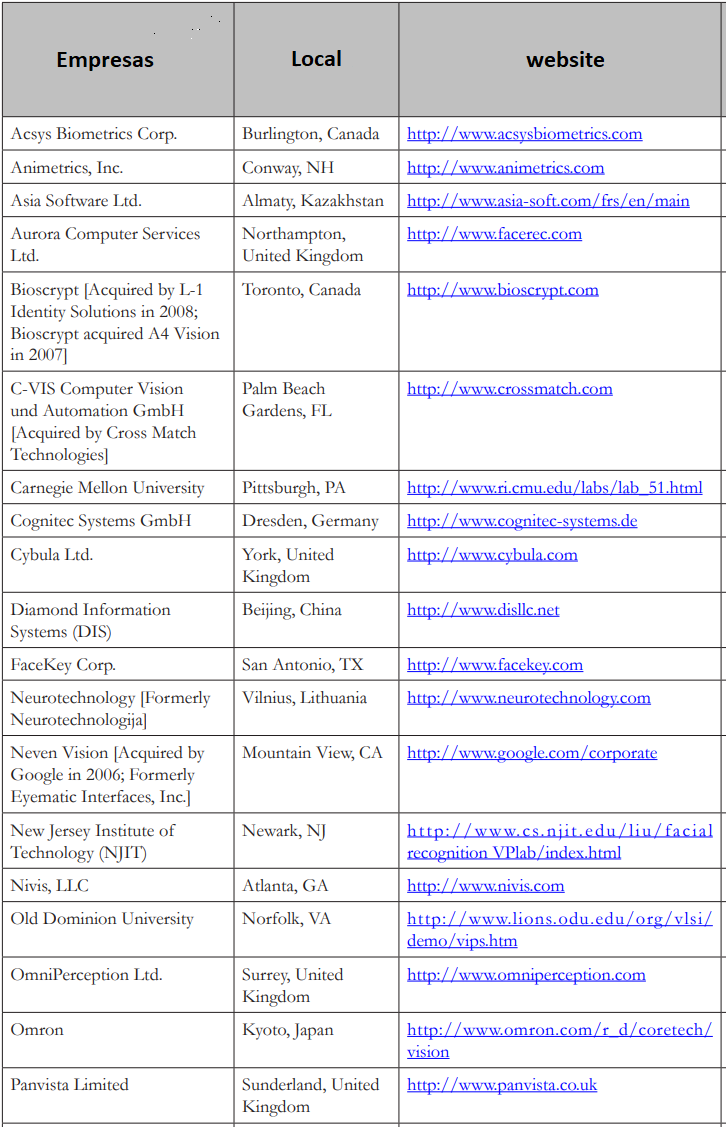
\includegraphics[width=.6\textwidth]{tabelaEmpresasRecog}
	\fonte{Adaptado de \cite{nstc_homeland}}
	\label{tabelaempresasrecog}
\end{table}



As pioneiras estão avançando exponencialmente no assuntos e gigantes como a Google e a Baidu já conseguem taxas de erros menores que humanos, com rapidez de verificação sem precedentes, como mostra a \autoref{statstoprecog}.

\vspace*{10cm}
\begin{figure}[h]
	\centering
	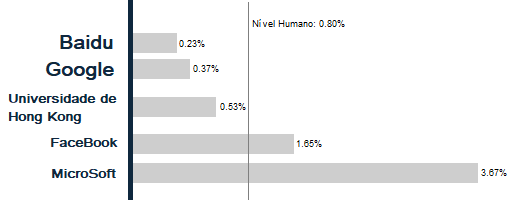
\includegraphics[width=.9\textwidth]{stats_toprecog}
	\caption{Comparação de sistemas de reconhecimento de faces em percentagem (\%) de erros}
	\fonte{Adaptado de \cite{stats_economy_compass_2017}}
	\label{statstoprecog}
\end{figure}


A \autoref{statstoprecog} mostra que a tecnologia da a gigante chinesa Baidu está liderando a corrida com apenas 0.23\% de taxa de erro, contra 0.37\% da empresa americana Google \cite{stats_economy_compass_2017}. Ambas já conseguiram ultrapassar as taxas alcançadas por seres humanos, que como mostra a \autoref{statstoprecog}, atinge a taxa de 0.8\% de erros. Como mostra \cite{stats_economy_compass_2017}, os humanos em geral não são uma fonte 100\% precisa para reconhecimento de faces. Humanos podem facilmente confundir pessoas, ou não reconhecê-las pela idade ou por mudança de aparência ou estilo, ou até esquecê-las.

No final de 2016, a Baidu implantou seu sistema em sua histórica “Cidade de Água”, substituindo totalmente o sistema de cartões e \textit{tickets} com 99\% de sucesso \cite{baidiu_theverge}, e já estão no processo de implantação em outros parques temáticos. Policiais chineses estão usando óculos de reconhecimento que verificam instantaneamente as faces de turistas e procurados. Com os armazenamentos e reconhecimentos dominando aplicativos de celulares e redes sociais, e a polícia com grande interesse forense no assunto, e outras infinitas possibilidades, obviamente esta tecnologia fará parte do dia a dia do nosso futuro, sendo assim é necessário estuda-la, entendê-la e desenvolvê-la.










